
% This LaTeX was auto-generated from MATLAB code.
% To make changes, update the MATLAB code and republish this document.

\documentclass{article}
\usepackage{graphicx}
\usepackage{color}

\sloppy
\definecolor{lightgray}{gray}{0.5}
\setlength{\parindent}{0pt}

\begin{document}

    
    
\section*{Gradient Descent}


\subsection*{Contents}

\begin{itemize}
\setlength{\itemsep}{-1ex}
   \item Gradient
   \item Gradient Descent
   \item Fail situation
   \item Plot contour
   \item Reference
\end{itemize}


\subsection*{Gradient}

\begin{par}
Gradient descent method is based on gradient
\end{par} \vspace{1em}
\begin{par}
$$ \nabla f  = \frac{\partial f}{\partial x_1 }\mathbf{e}_1 + \cdots +
\frac{\partial f}{\partial x_n }\mathbf{e}_n $$
\end{par} \vspace{1em}
\begin{par}
gradient always point to the asent direction
\end{par} \vspace{1em}


\subsection*{Gradient Descent}

\begin{par}
f is object function, and this is unconstrained
\end{par} \vspace{1em}
\begin{par}
$$\min_{x} f $$
\end{par} \vspace{1em}
\begin{verbatim}
f = (@(X) (exp(X(1,:)-1) + exp(1-X(2,:)) + (X(1,:) - X(2,:)).^2));
%f = (@(X) (sin(0.5*X(1,:).^2 - 0.25 * X(2,:).^2 + 3) .* cos(2*X(1,:) + 1 - exp(X(2,:))) ))
\end{verbatim}


\subsection*{Fail situation}

\begin{par}
Rosenbrock function Gradient descent/ascent algorithm zig-zags, because the gradient is nearly orthogonal to the direction of the local minimum in these regions. It's hard to convergence
\end{par} \vspace{1em}
\begin{par}
$$ f(x, y) = (1-x)^2 + 100 * (y - x^2) ^ 2 $$
\end{par} \vspace{1em}
\begin{verbatim}
%f = (@(X) (1-X(1,:)).^2 + 100 * (X(2,:) - X(1,:).^2).^2);
\end{verbatim}


\subsection*{Plot contour}

\begin{verbatim}
[X, Y] = meshgrid(-2:0.1:2);
XX = [reshape(X, 1, numel(X)); reshape(Y, 1, numel(Y))];
%surf(X, Y, reshape(f(XX), length(X), length(X)))
contour(X, Y, reshape(f(XX), length(X), length(X)), 50);

hold on;
\end{verbatim}

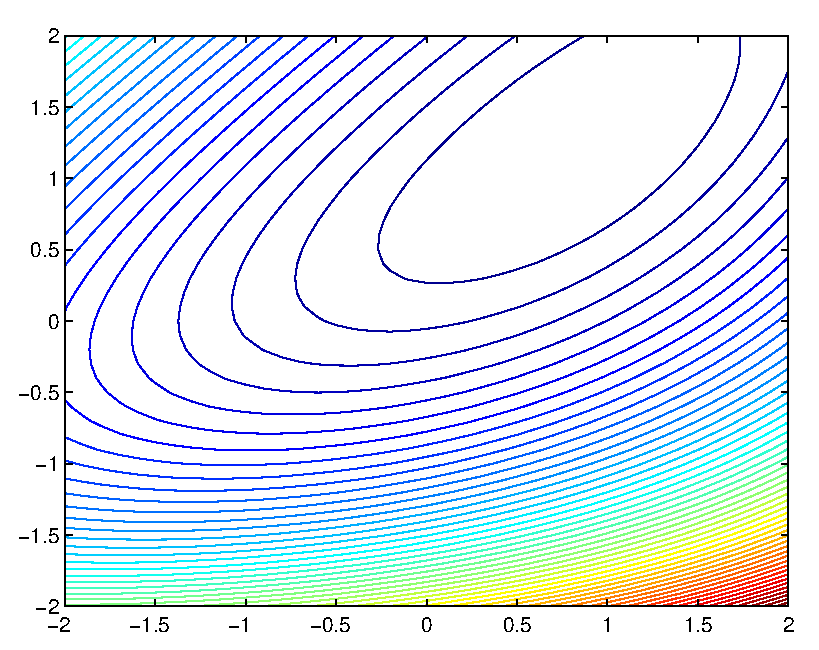
\includegraphics [width=4in]{test_01.eps}
\begin{par}
plot gradient of function
\end{par} \vspace{1em}
\begin{verbatim}
for i=1:5:length(XX)
    tmp = XX(:,i);
    g = gradient_of_function(f, tmp);
    %plot([tmp(1),tmp(1)+g(1)*0.02],[tmp(1),tmp(2)+g(1)*0.02]);
    quiver(tmp(1),tmp(2),g(1)*0.02,g(2)*0.02);
end
\end{verbatim}

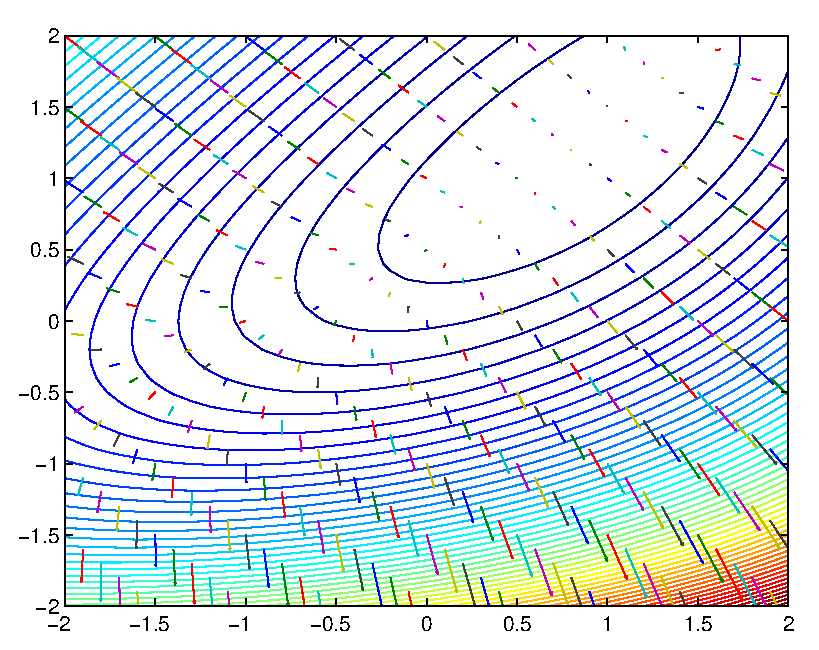
\includegraphics [width=4in]{test_02.eps}
\begin{par}
calculation
\end{par} \vspace{1em}
\begin{verbatim}
x0 = [-1; -1];
[x, v, h] = gradient(f, x0)

% built-in method
[x_in, v_in] = fminunc(f, x0)
\end{verbatim}

        \color{lightgray} \begin{verbatim}
x =

    0.7960
    1.2038


v =

    1.7974


h =

  Columns 1 through 7

   -1.0000   -1.0271   -0.4515    0.6432    0.8185    0.7755    0.7859
   -1.0000    0.4778    0.2130    1.0809    1.1279    1.1801    1.2059

  Columns 8 through 12

    0.7925    0.7963    0.7956    0.7959    0.7960
    1.2007    1.2024    1.2033    1.2039    1.2038

Warning: Gradient must be provided for trust-region algorithm;
  using line-search algorithm instead. 

Local minimum found.

Optimization completed because the size of the gradient is less than
the default value of the function tolerance.




x_in =

    0.7961
    1.2039


v_in =

    1.7974

\end{verbatim} \color{black}
    \begin{par}
plot descent steps
\end{par} \vspace{1em}
\begin{verbatim}
for i=2:length(h)
    tmp1 = h(:,i-1);
    tmp2 = h(:,i);
    quiver(tmp1(1),tmp1(2),tmp2(1)-tmp1(1),tmp2(2)-tmp1(2), 0, 'r','LineWidth',2)
end
\end{verbatim}

\includegraphics [width=4in]{test_03.eps}


\subsection*{Reference}

\begin{enumerate}
\setlength{\itemsep}{-1ex}
   \item \begin{verbatim}http://www.onmyphd.com/?p=gradient.descent\end{verbatim}
   \item Convex Optimization
   \item \begin{verbatim}https://en.wikipedia.org/wiki/Gradient\end{verbatim}
   \item \begin{verbatim}https://en.wikipedia.org/wiki/Gradient_descent\end{verbatim}
   \item \begin{verbatim}http://stronglyconvex.com/blog/gradient-descent.html\end{verbatim}
\end{enumerate}



\end{document}
    
